\documentclass{article}

% required packages
\usepackage[final]{neurips_2019}

\usepackage[linesnumbered,ruled,vlined]{algorithm2e}
\usepackage{hyperref}


\usepackage[utf8]{inputenc} % allow utf-8 input
\usepackage[T1]{fontenc}    % use 8-bit T1 fonts
\usepackage{hyperref}       % hyperlinks
\usepackage{url}            % simple URL typesetting
\usepackage{booktabs}       % professional-quality tables
\usepackage{amsfonts}       % blackboard math symbols
\usepackage{nicefrac}       % compact symbols for 1/2, etc.
\usepackage{microtype}      % microtypography

\usepackage{amsmath}
\usepackage{tikz}
\usepackage{subcaption} 
\usepackage{pgfplots}
\usepackage{filecontents}


\title{CE7490 Project: Benchmarking Algorithms for Weight Prediction in Weighted Signed Networks}

\author{
  Ruihang Wang\\
  G1901564E\\
  School of Computer Science Engineering\\
  Nanyang Technological University\\
  \texttt{ruihang001@e.ntu.edu.sg} 
  \And
  Meng Shen\\
  G1902579B\\
  School of Computer Science Engineering\\
  Nanyang Technological University\\
  \texttt{meng005@e.ntu.edu.sg}
  \And
  Yihang Li\\
  G1901408C\\
  School of Electrical and Electronic Engineering\\
  Nanyang Technological University\\
  \texttt{leah9704@gmail.com}
}

\begin{document}

\maketitle

\begin{abstract}
  A number of weighted signed networks (WSN) exist in our world while 
  many of them are incomplete. We are interested in finding the relationship
  and even capturing the scores between network users without direct connection.
  In this project, we first review a list of literatures that are
  related to signed social network. To predict weights of edges in 
  such networks, we gather a wide collection of existing edge weight
  prediction algorithms and test their performance on real-world datasets.
  Experiments of leaving one edge and leaving $N\%$ edeges are conducted,
  seperativly on each social network. The benchmarking results indicate
  that the combination of all the features of existing algorithms to learn
  a linear regression model outperforms the past techniques for edge weight
  prediction. To make it avaliable for interested researchers, we open-source our benchmark in 
  \url{https://github.com/RuihangWang/CE7490-OSN-Project}
\end{abstract}

\section{Introduction}

With the rapid development of information technology, social 
network has become a significant part of modern life. As 
huge volumes of messages reflecting opinions and attitudes 
flowing on the network, social network analysis gradually gains 
popularity in a wide range of fields, including political 
science, social psychology and business analysis. Social 
network analysis offers a tool to seek for insight through 
the structure of social networks, but is limited by its 
complexity. Users are developing rich relationships through 
networks while analysis tools are generally reducing the 
relationships to simple links. To cover the gap between 
simplicity of network simulation and complexity of real 
relationships is an interesting research topic. 

In social network, people show different attitudes towards 
connection to others. The richness of a social network contains 
positive and negative interactions. The main part of connections 
are positive ones, including connecting with friends, fans, and
followers. There also exist negative connections, including 
scammers, political enemy and opponents. These connections can 
be used to predict relationships between independent users. 
For example, a politician might look at such people as potential 
voters for him if he has strength in that particular topic of 
interest. In the same vein, we might wish to estimate how much 
a person P1 agrees/disagrees with people who are already 
positive or negative about a product in order to quantify if 
they are more likely to be target customers of the product. 
Moreover, edge weight prediction may be useful to improve 
traditional tasks in signed networks such as node ranking
\cite{shahriari2014ranking}, anomaly detection\cite{Kmumar2014}
\cite{Wu:2016:TMR:2835776.2835816}, network 
analysis\cite{Kumar:2016:SDS:2872518.2889391}
\cite{leskovec2010signed}, community detection
\cite{PhysRevE.80.036115}, information diffusion
\cite{Shafaei_2014} \cite{Li2014} and sentiment 
prediction\cite{west2014}. Therefore, the prediction of edge 
weights in WSNs can be advantageous in various tasks, both 
when WSNs are explicit and implicit.

To better understand theories and master practical skills, 
we investigate and implement a common set of algorithms and 
evaluate their performance on real-world datasets. 
The rest of the paper is structured as follows: Section 2 
presents related work in this topic. Section 3 describes the 
overview of our project. Section 4 formulates the problem of 
weight prediction in weighted signed networks. Section 5 
conducted experiments on real-world datasets using different 
algorithms. Section 6 evaluates the performance of all tested 
methods. The conclusion is summarized in Section 7.

\section{Related Work}
\subsection{Edge Sign Prediction in SSNs}
In the early stage, the work in
SSN mainly based on balance and status. The first of these 
theories is structural balance theory, which originated in 
social psychology in the mid-20th-century. As formulated by 
Heider in the 1940s\cite{heider1940}, and subsequently cast 
in graph-theoretic language by Cartwright and 
Harary\cite{Cartwright1956-CARSBA-4}, structural balance 
considers the possible ways in which triangles on three 
individuals can be signed, and posits that triangles with 
three positive signs and those with one positive sign are 
more plausible — and hence should be more prevalent in real 
networks — than triangles with two positive signs or none. 
Balanced triangles with three positive edges exemplify the 
principle that “the friend of my friend is my friend,” whereas 
those with one positive and two negative edges capture the 
notions that “the friend of my enemy is my enemy,” 
“the enemy of my friend is my enemy,” and 
“the enemy of my enemy is my friend.” 
Structural balance theory has been developed extensively 
in the time since this initial work\cite{wasserman1994social}, 
including the formulation of a variant “weak structural balance” 
proposed by Davis in the 1960s \cite{Davis1967}as a way of 
eliminating the assumption that “the enemy of my enemy is my 
friend”. Weak structural balance posits that only triangles 
with exactly two positive edges are implausible in real 
networks, and that all other kinds of triangles should be 
permissible.

Balance theory can be viewed as a model of likes and dislikes. 
However, as Guha et al. observe in the context of 
Epinions\cite{Guha:2004:PTD:988672.988727}, a signed link from 
P1 to P2 can have more than one possible interpretation, 
depending on P1’s intention in creating the link. 
In particular, a positive link from P1 may mean, 
“P2 is my friend,” but it also may mean, “I think P2 has higher 
status than I do.” Similarly, a negative link from P1 to P2 may
 mean “P2 is my enemy” or “I think P2 has lower status than 
 I do.”

Later work have developed features and models to predict the 
sign of an edge random-walk and trust-propagation 
algorithms\cite{Dubois}\cite{Guha:2004:PTD:988672.988727}, 
and using social interaction information for prediction
\cite{Yang2012}\cite{Tang:2016:SSN:2988524.2956185}. Metric 
Multidimensional Scaling (MDS) assigns an m-dimensional 
position to vertices in a SSN or WSN to minimize ‘stress’, 
based on extended balance theory\cite{Qian:2014:FTD:2639948.2628438}. 
It then uses the metric distance between two vertices to 
predict the sign of an edge between them. All of these papers 
predict edge sign in unweighted SSNs, while fairness and 
goodness method predicts the weight of an edge along with its 
sign. 

\subsection{Edge Weight Prediction in Social Networks}
There is substantial work on predicting edge weights in unsigned social 
networks. Communication based features have been shown to be 
very important in quantifying the edge weights between 
users\cite{Gilbert:2012:PTS:2145204.2145360}\cite{Gilbert:2009:PTS:1518701.1518736}
\cite{Xiang:2010:MRS:1772690.1772790}\cite{Kahanda2009}, but 
since we only have the WSN without any communication information, 
we compare with non-communication based techniques. These 
include baselines such as reciprocal edge weight\cite{Gilbert:2012:PTS:2145204.2145360} 
and triadic balance and status measures\cite{Gilbert:2009:PTS:1518701.1518736}
\cite{Sintos:2014:UST:2623330.2623664}. Two popular unsupervised 
algorithms are EigenTrust\cite{Kamvar:2003:EAR:775152.775242} 
and TidalTrust\cite{Katz2006}. EigenTrust calculates a global 
value of trust for each vertex by finding the left eigenvector 
of a normalized trust matrix. TidalTrust calculates the trust 
from a source to a sink, by recursively propagating trust via 
the sink’s predecessors till it reaches the source. A very 
recent work in this direction is trustingness and 
trustworthiness\cite{Roy2016}. However, these papers deal with 
edge weight prediction in unsigned social networks, while WSN 
is a new problem deriving from SSN. So in this paper, these 
techniques are implemented and compared with fairness and goodness 
method as benchmark models.

\section{Project Overview}
In this project, we extensively investigate and experiment methods for edge weight prediction in WSNs. All algorithms are tested and evaluated on published real-world datasets. Moreover, we try our best to improve the performance on some traditional methods. The finished works are summarized as follows:

\begin{enumerate}
	\item Literature review on OSN and select a topic about predicting weight of edges for WSN.
	
	\item Investigated the state-of-the-art algorithms \emph{fairness-goodness} in\cite{kumar2016edge} and  studied a common set of baselines for weight prediction.
	
	\item Conducted experiments on each algorithm and reproduce the results mentioned in original paper using real-world dataset.
  
  \begin{itemize}
    \item \emph{Experimental 1 -   Removing one edge prediction}: 
    When we remove one of the edges from the network and try to 
    predict it from the rest of network structure one at a time, 
    we compared fairness and goodness metrics with other typical 
    methods and noticed that fairness and goodness method produces 
    almost the best result. 
	
    \item \emph{Experimental 2 -  Removing $N \%$-out edge prediction}: 
    When we remove $N\%$ of the edges from the network and try to 
    predict them from each of the individual features, we see 
    that in all cases, fairness and goodness metrics are the best.
  \end{itemize}
  
  \item  Evaluated results of different methods and summarized the conclusions of this project.
	
\end{enumerate}

\section{Algorithms}

In this section, we investigate a common set of algorithms
associated with signed social networks. The procedures and
formulas of these algorithms for edge weight prediction are 
discussed in details. 

% !TeX root = ../OSN.tex

\subsection{Fairness and Goodness}

The fairness and goodness models is the state-of-art algorithm for 
edge weight prediction created by Srijan Kumar in \cite{kumar2016edge}.
The metrics are based on the intuition that a 'fair' or 'reliable' 
rater should give a user the rating that it deserves, while an 'unfair'
one would deviate from that value. Hence, the ratings given by unfair 
raters should be given low importance, while ratings given by fair 
raters should be considered important. From the description above,
we can see that the fairness and goodness metrics are dependent on each
other.

To investigate this method, we first need to understand the defination
of fairness and goodness from a mathmatical perspective. According to 
the author, the fairness and goodness dependency should satisfy the 
following definations.

\emph{\textbf{Goodness defination}}: The goodness axiom states that 
vertices with higher fairness have higher impact on the vertices they rate.
Formally, let $u_1$ and $u_2$ denote two vertices having identical ego-in-networks,
and $h$ be the $1$-to-$1$ mapping between the two ego-in-networks. If
$f(v) = f(h(v)), \forall v \in in^-(u_1)$, and $f(v) \geq f(h(v)), \forall v \in in^+(u_1)$,
then $g(u_1) \geq g(u_2)$. Conversely, if $f(v) = f(h(v)), \forall v \in in^+(u_1)$, 
and $f(v) \geq f(h(v)), \forall v \in in^-(u_1)$, then $g(u_1) \leq g(u_2)$

\emph{\textbf{Fairness defination}}: The fairness axiom states that 
a vertex is more fair than another if it gives ratings closer to the rating
deserved by the recipent.
Formally, let $u_1$ and $u_2$ denote two vertices having identical ego-out-networks,
and $h$ be the $1$-to-$1$ mapping between the two ego-out-networks.
If $|W_{u_1}(u_1, k)-g(k)| \leq |W_{u_2}(u_2, h(k))-g(h(k))|, \forall k \in out(u_1)$,
then $f(u_1) \geq f(u_2)$.

\emph{\textbf{Metrics Equations}}: From the above defination, the goodness ($g(v)$) and fairness ($f(u)$) are 
iteratively calculated by:

\begin{equation}
    g(v) = \frac{1}{|in(v)|}\sum_{u \in in(v)}f(u) \times W(u,v)
\end{equation}

\begin{equation}
    f(u) = 1 - \frac{1}{|out(v)|}\sum_{v \in out(u)}\frac{W(u,v)-g(v)}{R}
\end{equation}

where $R=2$\footnote{If edge weights and goodness range over $[-\ell, \ell]$, then $R = 2\ell$},
$in(v)$ is a set of nodes that preceed $v$, $out(u)$ is 
a set of nodes that succeed $u$, and $W(u,v)$ is the weight
of ($u,v$). We say that two nodes $u$ and $v$ have the identical
ego-in-network if $|in(u)| = |in(v)|$, Similarly, the ego-out-network
is defined by the same rule. Therefore, the algorithm for calculating
fairness and goodness is implemented as below:

\begin{algorithm}
    \KwIn{A WSN $G = (V,E,W)$}
    \KwOut{Fairness and Goodness scores for all vertices in $V$}
    Let $f^0(u) = 1$ and $g^0(u) = 1$, $\forall u \in V$ \\
    $t = -1$ \\
    \Repeat{$\sum_{u \in V}|f^{(t+1)}(u)-f^t(u)| > \epsilon$ \quad or \quad $\sum_{u \in V}|g^{(t+1)}(u)-g^t(u)| > \epsilon$}{
        $t = t+1$ \\
        $g^{(t+1)}(v) = \frac{1}{|in(v)|}\sum_{u \in in(v)}f^t(u) \times W(u,v)$, $\forall v \in V$\\
        $f^{(t+1)}(u) = 1 - \frac{1}{2|out(v)|}\sum_{v \in out(u)}W(u,v)-g^{(t+1)}(v)$, $\forall u \in V$\\
    }
    \Return{$g^{(t+1)}(u) \quad and \quad f^{(t+1)}(u)$}\\
    \caption{Fairness and Goodness algorithm}
\end{algorithm}

Figure 1 shows the fairness and goodness distribution for all 
the vertices in the \textbf{BTCAlphaNet}. We can see that most vertices
in the network have very high fairness ($90\%$ above 0.8 score; mean score = 0.94)
meaning that most of the users are fair, but some vertices are not.
For goodness, most vertices have low positive score ($80\%$ have 
score between 0 and 0.3), while a considerable fraction are 
considered ‘not good’ ($14\%$ have negative score, and $5\%$ have 
goodness below -0.5). Similar observations hold for other 
networks.

Based on the definations and equations given by the original paper, we reproduce
the edge weight prediction by taking the product of the fairness and
goodness of each node. Thus, the predicted weight of ($u,v$) is given by:
\begin{equation}
    W(u,v) = f(u) \times g(v)
\end{equation}
where $W(u,v)$ depends on both the fairness $f(u)$ of the edge 
generator ($u$) and the goodness of the edge recipent ($v$).

\begin{filecontents*}{F_distribution_BTCAlphaNet.csv}
$f:$ Fairness score, Frac. of vertices with Fairness $f$
0.00E+00,0.00E+00
5.00E-02,0.00E+00
1.00E-01,0.00E+00
1.50E-01,0.00E+00
2.00E-01,0.00E+00
2.50E-01,0.00E+00
3.00E-01,4.25E-04
3.50E-01,1.13E-03
4.00E-01,1.84E-03
4.50E-01,1.98E-03
5.00E-01,5.24E-03
5.50E-01,9.07E-03
6.00E-01,7.79E-03
6.50E-01,6.94E-03
7.00E-01,1.08E-02
7.50E-01,2.00E-02
8.00E-01,4.31E-02
8.50E-01,1.56E-01
9.00E-01,3.95E-01
9.50E-01,3.41E-01
\end{filecontents*}

\begin{filecontents*}{F_distribution_OTCNet.csv}
$f:$ Fairness score, Frac. of vertices with Fairness $f$
0.00E+00,0.00E+00
5.00E-02,0.00E+00
1.00E-01,0.00E+00
1.50E-01,0.00E+00
2.00E-01,0.00E+00
2.50E-01,2.81E-04
3.00E-01,7.49E-04
3.50E-01,1.50E-03
4.00E-01,3.00E-03
4.50E-01,3.84E-03
5.00E-01,8.24E-03
5.50E-01,1.38E-02
6.00E-01,1.14E-02
6.50E-01,1.08E-02
7.00E-01,1.55E-02
7.50E-01,2.75E-02
8.00E-01,5.05E-02
8.50E-01,1.43E-01
9.00E-01,3.60E-01
9.50E-01,3.51E-01
\end{filecontents*}

\begin{filecontents*}{F_distribution_RFAnet.csv}
$f:$ Fairness score, Frac. of vertices with Fairness $f$
0.00E+00,0.00E+00
5.00E-02,0.00E+00
1.00E-01,0.00E+00
1.50E-01,0.00E+00
2.00E-01,0.00E+00
2.50E-01,0.00E+00
3.00E-01,0.00E+00
3.50E-01,5.47E-05
4.00E-01,5.47E-05
4.50E-01,2.19E-04
5.00E-01,7.11E-04
5.50E-01,1.70E-03
6.00E-01,3.94E-03
6.50E-01,7.66E-03
7.00E-01,1.67E-02
7.50E-01,4.14E-02
8.00E-01,1.20E-01
8.50E-01,3.09E-01
9.00E-01,3.30E-01
9.50E-01,1.69E-01
\end{filecontents*}

\begin{filecontents*}{G_distribution_BTCAlphaNet.csv}
$g:$ Goodness score, Frac. of vertices with Goodness $g$
-1.00E+00,2.67E-03
-9.50E-01,6.95E-03
-9.00E-01,2.94E-03
-8.50E-01,1.07E-03
-8.00E-01,5.35E-04
-7.50E-01,8.02E-04
-7.00E-01,1.60E-03
-6.50E-01,2.14E-03
-6.00E-01,2.67E-03
-5.50E-01,1.07E-03
-5.00E-01,5.08E-03
-4.50E-01,4.28E-03
-4.00E-01,3.74E-03
-3.50E-01,2.67E-03
-3.00E-01,3.48E-03
-2.50E-01,5.35E-03
-2.00E-01,4.28E-03
-1.50E-01,2.14E-03
-1.00E-01,1.52E-02
-5.00E-02,7.22E-03
0.00E+00,1.31E-02
5.00E-02,4.36E-01
1.00E-01,1.48E-01
1.50E-01,1.58E-01
2.00E-01,5.40E-02
2.50E-01,4.73E-02
3.00E-01,1.20E-02
3.50E-01,1.58E-02
4.00E-01,8.82E-03
4.50E-01,9.62E-03
5.00E-01,4.81E-03
5.50E-01,2.41E-03
6.00E-01,2.14E-03
6.50E-01,1.34E-03
7.00E-01,8.02E-04
7.50E-01,2.14E-03
8.00E-01,2.14E-03
8.50E-01,1.60E-03
9.00E-01,3.21E-03
9.50E-01,1.87E-03
\end{filecontents*}

\begin{filecontents*}{G_distribution_OTCNet.csv}
$g:$ Goodness score, Frac. of vertices with Goodness $g$
-1.00E+00,2.91E-03
-9.50E-01,1.75E-02
-9.00E-01,4.79E-03
-8.50E-01,2.57E-03
-8.00E-01,2.91E-03
-7.50E-01,1.88E-03
-7.00E-01,4.28E-03
-6.50E-01,4.96E-03
-6.00E-01,5.30E-03
-5.50E-01,3.76E-03
-5.00E-01,6.33E-03
-4.50E-01,7.53E-03
-4.00E-01,8.90E-03
-3.50E-01,5.30E-03
-3.00E-01,5.99E-03
-2.50E-01,8.73E-03
-2.00E-01,1.47E-02
-1.50E-01,6.16E-03
-1.00E-01,1.75E-02
-5.00E-02,9.41E-03
0.00E+00,1.28E-02
5.00E-02,4.46E-01
1.00E-01,1.30E-01
1.50E-01,1.32E-01
2.00E-01,4.41E-02
2.50E-01,3.94E-02
3.00E-01,9.92E-03
3.50E-01,1.37E-02
4.00E-01,5.99E-03
4.50E-01,9.07E-03
5.00E-01,2.91E-03
5.50E-01,1.71E-03
6.00E-01,1.54E-03
6.50E-01,1.03E-03
7.00E-01,1.20E-03
7.50E-01,1.37E-03
8.00E-01,8.56E-04
8.50E-01,1.03E-03
9.00E-01,2.40E-03
9.50E-01,1.54E-03
\end{filecontents*}

\begin{filecontents*}{G_distribution_RFAnet.csv}
$g:$ Goodness score, Frac. of vertices with Goodness $g$
-1.00E+00,2.91E-03
-9.50E-01,1.75E-02
-9.00E-01,4.79E-03
-8.50E-01,2.57E-03
-8.00E-01,2.91E-03
-7.50E-01,1.88E-03
-7.00E-01,4.28E-03
-6.50E-01,4.96E-03
-6.00E-01,5.30E-03
-5.50E-01,3.76E-03
-5.00E-01,6.33E-03
-4.50E-01,7.53E-03
-4.00E-01,8.90E-03
-3.50E-01,5.30E-03
-3.00E-01,5.99E-03
-2.50E-01,8.73E-03
-2.00E-01,1.47E-02
-1.50E-01,6.16E-03
-1.00E-01,1.75E-02
-5.00E-02,9.41E-03
0.00E+00,1.28E-02
5.00E-02,4.46E-01
1.00E-01,1.30E-01
1.50E-01,1.32E-01
2.00E-01,4.41E-02
2.50E-01,3.94E-02
3.00E-01,9.92E-03
3.50E-01,1.37E-02
4.00E-01,5.99E-03
4.50E-01,9.07E-03
5.00E-01,2.91E-03
5.50E-01,1.71E-03
6.00E-01,1.54E-03
6.50E-01,1.03E-03
7.00E-01,1.20E-03
7.50E-01,1.37E-03
8.00E-01,8.56E-04
8.50E-01,1.03E-03
9.00E-01,2.40E-03
9.50E-01,1.54E-03
\end{filecontents*}

\begin{filecontents*}{residual_BTCAlphaNet.csv}
Iteration Number, Fairness, Goodness
1,19.26203548,52.77075812
2,0.899897124,2.73121104
3,0.120910925,0.30603546
4,0.023750527,0.052002113
5,0.005540736,0.010606994
6,0.001405605,0.002415427
7,0.000371799,0.000585373
8,0.000100602,0.000146979
9,2.76E-05,3.77E-05
10,7.66E-06,9.85E-06
11,2.14E-06,2.60E-06
12,6.02E-07,6.94E-07
\end{filecontents*}

\begin{filecontents*}{residual_OTCNet.csv}
Iteration Number, Fairness, Goodness
1,34.46583923,102.2916736
2,2.390951436,6.965249258
3,0.389480015,1.059994363
4,0.096409505,0.239180648
5,0.027072632,0.062646945
6,0.007785908,0.017275492
7,0.002266912,0.004895509
8,0.000664334,0.001409055
9,0.000195759,0.000410127
10,5.81E-05,0.000120386
11,1.73E-05,3.58E-05
12,5.18E-06,1.07E-05
13,1.55E-06,3.23E-06
14,4.65E-07,9.70E-07
\end{filecontents*}

\begin{filecontents*}{residual_RFAnet.csv}
Iteration Number, Fairness, Goodness
0,753.9504452,0
1,62.52521643,78.67886092
2,1.698504052,2.662806214
3,0.090952342,0.186354032
4,0.007766118,0.0194343
5,0.00091073,0.002441522
6,0.000124147,0.000333286
7,1.82E-05,4.77E-05
8,2.80E-06,7.08E-06
9,4.50E-07,1.10E-06
10,7.52E-08,1.77E-07
\end{filecontents*}

\begin{figure}[htbp]
    \centering
    \begin{tikzpicture}
    \pgfplotsset{every axis legend/.append style={at={(-0.2,-0.8)},anchor=south},every axis y label/.append style={at={(0.1,0.5)}}}
    \begin{axis}[title= Fairness Distribution ,xlabel=$f:$ Fairness score, ylabel=Frac. of vertices with Fairness $f$,xtick ={0,0.2,0.4,0.6,0.8,1},legend columns=5,legend style={font=\tiny},font=\tiny,width=5cm]
    \addplot [very thick,color=blue,mark=None] table [x=$f:$ Fairness score, y=Frac. of vertices with Fairness $f$, col sep=comma] {F_distribution_BTCAlphaNet.csv};
    \end{axis}
    \end{tikzpicture}
    \begin{tikzpicture}
    \pgfplotsset{every axis legend/.append style={at={(-0.2,-0.8)},anchor=south},every axis y label/.append style={at={(0.1,0.5)}}}
    \begin{axis}[title= Goodness Distribution ,xlabel=$g:$ Goodness score, ylabel=Frac. of vertices with Goodness $g$,xtick ={-1,-0.5,0,0.5,1},legend columns=5,legend style={font=\tiny},font=\tiny,width=5cm]
    \addplot [very thick,color=red,mark=None] table [x=$g:$ Goodness score, y=Frac. of vertices with Goodness $g$, col sep=comma] {G_distribution_BTCAlphaNet.csv};
    \end{axis}
    \end{tikzpicture}
    \begin{tikzpicture}
    \pgfplotsset{every axis legend/.append style={at={(0.7,0.65)},anchor=south},every axis y label/.append style={at={(0.1,0.5)}}}
    \begin{semilogyaxis}[title= Residual ,xlabel=Iteration Number, ylabel=Change in Value,xtick =data,legend columns=1,legend style={font=\tiny},font=\tiny,width=5cm]
    \addplot table [x=Iteration Number, y=Fairness, col sep=comma] {residual_BTCAlphaNet.csv};
    \addplot table [x=Iteration Number, y=Goodness, col sep=comma] {residual_BTCAlphaNet.csv};
    \legend{$$Fairness, $$Goodness}
    \end{semilogyaxis}
    \end{tikzpicture}
    \caption{BTCAlphaNet}
\end{figure}

% !TeX root = ../OSN.tex
\subsection{Reciprocal}
As a baseline of weight prediction, reciprocal algorithm takes the 
weight of ($v,u$) as equal to the weight of ($u,v$). When the reciprocal edge 
doesn't exist, the weight of that edge is set to 0. Therefore, the weight of ($u,v$)
is predicted by:

\begin{equation}
W(u,v) =
\begin{cases}
W(v,u),& \text{if $u \rightarrow v$ exist} \\
0,&  \text{otherwise}
\end{cases}
\end{equation}







% !TeX root = ../OSN.tex
\subsection{Triadic balance}
This definition is derived directly from
balance theory according to \cite{}. The algorithm takes the average product of edge weights for all incomplete triads
that the edge ($u,v$) is a part of. Incomplete triads are triads that would form involving
edge ($u,v$) after it is created. To be specific, let $U_n$ and $V_n$ denotes the set of
neighbors of vertex $u$ and $v$, repectively. To find all possible triads, vertexes with
both connections of $u$ and $v$ are obtained by $N = U_n \cap V_n$. When $N = \emptyset$,
the weight of ($u,v$) is set to 0. Then, the weight of ($u,v$)
is predicted by:

\begin{equation}
W(u,v) = 
\begin{cases}
\frac{\sum_{n\in N}W(u,n)+W(n,u)+W(v,n)+W(n,v)}{M}, & \text{if $N \neq \emptyset$} \\
0, & \text{otherwise}
\end{cases}
\end{equation}

where M is number of vertexes in set $N$, $W(u,n), W(n,u), W(v,n), W(n,v)$ are weights of each edge connected
to $u$ or $v$ of vertexes in set $N$, repectively.

% !TeX root = ../OSN.tex

\subsection{Triadic Status}

Imaging there are two nodes named $A$ and $B$, and they are unlinked. What we want to do is to predict the weight of the edge from $A$ to $B$. Suppose that there is another node $X$, and $(A, B, X)$ compose a triangle once $A$ and $B$ are linked. Overall, there are four different triangle-links, as the edge between $X$ and $A$ can go in either direction and similarly for the edge between $X$ and $B$, if the sign of weight is not considered.

\begin{figure}[htbp]
\centering
	\begin{subfigure}{0.2\textwidth}
		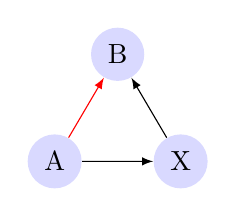
\begin{tikzpicture}
		[scale=0.8,every node/.style={circle,fill=blue!15}]
		  \node (A) at (1,1) {A};
		  \node (B) at (2,2.7)  {B};
		  \node (X) at (3,1)  {X};
		  \draw[->, >=latex, red] (A) edge (B);
		  \draw[->, >=latex] (A) edge (X);
		  \draw[->, >=latex] (X) edge (B);
		\end{tikzpicture}
		\caption{t1}
		\label{t1}
	\end{subfigure}
	\begin{subfigure}{0.2\textwidth}

		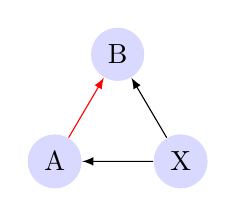
\begin{tikzpicture}
		[scale=0.8,every node/.style={circle,fill=blue!15}]
		\node (A) at (1,1) {A};
		\node (B) at (2,2.7)  {B};
		\node (X) at (3,1)  {X};
		\draw[->, >=latex, red] (A) edge (B);
		\draw[->, >=latex] (X) edge (A);
		\draw[->, >=latex] (X) edge (B);
		\end{tikzpicture}
		\caption{t2}
		\label{t2}
	\end{subfigure}
	\begin{subfigure}{0.2\textwidth}

		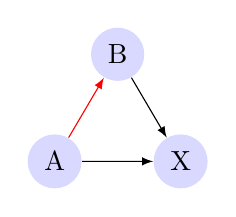
\begin{tikzpicture}
		[scale=0.8,every node/.style={circle,fill=blue!15}]
		\node (A) at (1,1) {A};
		\node (B) at (2,2.7)  {B};
		\node (X) at (3,1)  {X};
		\draw[->, >=latex, red] (A) edge (B);
		\draw[->, >=latex] (A) edge (X);
		\draw[->, >=latex] (B) edge (X);
		\end{tikzpicture}
		\caption{t3}
		\label{t3}
	\end{subfigure}
	\begin{subfigure}{0.2\textwidth}

		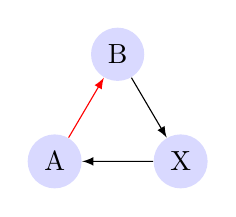
\begin{tikzpicture}
		[scale=0.8,every node/.style={circle,fill=blue!15}]
		  \node (A) at (1,1) {A};
		  \node (B) at (2,2.7)  {B};
		  \node (X) at (3,1)  {X};
		  \draw[->, >=latex, red] (A) edge (B);
		  \draw[->, >=latex] (X) edge (A);
		  \draw[->, >=latex] (B) edge (X);
		\end{tikzpicture}
		\caption{t4}
		\label{t4}
	\end{subfigure}
	\caption{Triadic Status}
	\label{Triadic Status Figure}
\end{figure}

And we predict the weight of the edge $(A, B)$ using three rules:

\begin{enumerate}

\item In Graph t1, the predicted weight of the transitive edge is the sum of the two non-transitive edge weights.

\item In Graph t2 and t3, the predicted weight of a non-transitive edge is the difference of the transitive and the other non-transitive edge weights. 

\item In Graph t4, since it is a cyclic triad, the weight of the missing edge is the negative of the sum of other two edge weights.

\end{enumerate}

In the end, we take the average of predicted weights over all triadic-links that these two nodes are a part of.





% !TeX root = ../OSN.tex

\subsection{Status Theory}

Status theory is derived from \cite{Status}. The prediction made by this measure
is the difference between the status of vertex $u$ and vertex $v$. The status
$\sigma (i)$ of a vertex $i$ is defined as $\sigma (i) = |W^+_{in}(i)| - |W^-_{in}(i)| + |W^-_{out}(i)| - |W^+_{out}(i)|$.
Status increases when receiving positive incoming edges and generating negative 
outgoing edges to other vertices, while decreases when receiving negative edges 
and generating outgoing positive edges. Difference in status measures how much ‘higher’ $u’$s 
status is compared to $v’$s.


% !TeX root = ../OSN.tex

\subsection{Bias and Deserve}
This method is proposed by Mishra and Bhattacharya in \cite{}.
To compute "bias" and "deserve", we should first normalize the ratings (weights),
and keep them in the range of [-1, 1] where 0 is a neutral opinion. Then, we say node $u$ gives a trust-score
of $w_ij$ to node $v$ for a given rating of ($u, v$). The two attributes of a node are 
defined by:

\begin{itemize}
	\item \emph{Bias}: This reflects the expected weight of an outgoing edge.  
	\item \emph{Deserve}: This reflects the expected weight of an incoming edge from an unbiased vertex.
\end{itemize}

Let $d^o(u)$ denotes the set of all outgoing edges from vertex $u$ and likewise,
$d^i(u)$ denotes the set of all incoming links to node $u$. Then, bias (BIAS) and
deserve (DES) are iteratively computed as:

\begin{equation}
    BIAS^{(t+1)}(u)=\frac{1}{å2|d^o(u)|}\sum_{v \in d^o(u)}[W(u,v) - DES^t(v)]
\end{equation}

\begin{equation}
    DES^{(t+1)}(u)=\frac{1}{å2|d^i(u)|}\sum_{v \in d^i(u)}[W(v,u)(1 - X^t(v,u))]
\end{equation}

where $X^t(v,u) = max\{0, BIAS^t(v) \times W(v,u)\}$. The interative formulations
of bias and deserve allow us to predict the weight of (u,v) based on the deserve
value $DES(v)$ of vertex $v$. Thus, the weight is directly predicted by:

\begin{equation}
    W(u,v) = DES(v)
\end{equation}

% !TeX root = ../OSN.tex

\subsection{Page Rank}

We first compute Page Rank ($\omega PR$) value of every vertex(k) in an unsigned graph according to \cite{brin1998anatomy}:

\begin{equation}
\omega PR(k) = \frac{1 - \alpha}{\left | V \right|} + \alpha \sum_{z\in in(k)}\frac{\omega PR(z) * W(z,k)}{\left | out(z) \right |}
\end{equation}

$\alpha$ is the probability called damping factor meaning a person will continue clicking on links(travelling in graph), and we set $\alpha$ to 0.85. $\left |V\right |$ is the number of all nodes. Eventually, $\omega PR(k)$ will converge to the probability that a person will go and stay at node k.

Then we compute edge weight of $(u,v)$ using weighted average of PageRank values:

\begin{equation}
W(u,v) = \frac{\sum_{z\in out(u)} \omega PR(z)*W(u,z) + \sum_{z\in in(v)} \omega PR(z)*W(z,v)}
{\sum_{z\in out(u)}\omega PR(z) + \sum_{z\in in(v)}\omega PR(z)}
\end{equation}



% !TeX root = ../OSN.tex

\subsection{Signed-Hits}

The prediction is computed by using a modified version of HITS for signed network, called Signed-HITS\cite{shahriari2014ranking}. Signed-HITS will compute the hub and authority scores of every node separately on positive graph(all edges' weights are positive) and negative graph, using the equation:

\begin{equation}
\begin{aligned}
h^+(u) = \sum_{v\in out^+(v)}{a^+(v)} ; a^+(u) = \sum_{v\in ^+(u)}{h^+(v)}\\
h^-(u) = \sum_{v\in out^-(v)}{a^-(v)} ; a^-(u) = \sum_{v\in ^-(u)}{h^-(v)}
\end{aligned}
\end{equation}

after convergence, we assign the authority score $a(u)=a^+(u)-a^-(u)$ and hub score $h(u)=h^+(u)-h^-(u)$ to each vertex $u$. Authority scores estimate the node value based on the incoming links, while hub scores estimate the node value based on outgoing links. However, the paper\cite{kumar2016edge} didn't deliver the method to compute edge weight by using the authority score and hub score. Again, we use weighted average to compute the weight prediction:

\begin{equation}
W(u,v) = \frac{h(u)*\sum_{z\in out(u)} W(u,z) + a(v)*\sum_{z\in in(v)} W(z,v)}{h(u) * |V_{z\in out(u)}| + a(v) * |V_{z\in in(v)}|}
\end{equation}

In this equation, we use $h(u)$ to be the weight of all out-going edges and $a(v)$ to be the weight of all in-coming edges. The reason is that $h(u)$ represents the node value based on out-going edges. So the predicted weight of out-edges from $u$ should be higher if $h(u)$ is high. Likewise, the predicted weight of in-edges into $v$ should be higher if $a(v)$ is high.

% !TeX root = ../OSN.tex

\subsection{Linear Regression}

In this experiment, we use a linear regression model to predict the weight of edge. Our features are generated from some algorithms mentioned above. First, the test edge $e_t$ whose weight is to be predicted is removed from the network. Second, we remove the second edge $e_s$ and predict the weight of $e_s$ from the rest of the edges. And the predicted value of $e_s$ will be the feature and the true value of $e_s$ will be the ground truth. The second step is done multiple times to generate enough samples for training. After training, we use this model to predict the value of the removed edge $e_t$.

\section{Performance Evaluation}

% !TeX root = ../OSN.tex

We implemented two series of experiments to evaluate the 
performance of fairness and goodness method on three public 
WSN dataset mentioned above. 

Experiment1:leave-one-out prediction
In these experiments, one weighted edge is removed at a time 
and nine algorithms are implemented to predict the weight of 
test edge, simulating the situation where we want to calculate 
the weight of a non-existed edge. The root-mean-square error 
(RMSE) and Pearson correlation coefficient (PCC) are calculated 
in each loot and the average result is shown in table \ref{table1}. 
Fairness and goodness method achieved almost the best 
performance among all datasets and showed robustness. 
The linear regression result trained by all other features 
is the best one. 

Experiment2:leave-N\%-out prediction
In this part, we removed a larger number of edges to further 
evaluate the performance of F\&G algorithm. We randomly selected 
N\% of the edges, remove them as test edges and predict their 
weight from the rest of network. The value of N range from 10 
to 90 with a step of 10. Figure\ref{figure3}, Figure\ref{figure4} and 
Figure\ref{figure5} showed average RMSE and PCC results in 
the three datasets. F\&G method beats most of the algorithms 
and linear regression method showed robustness and performed 
nearly the best in all datasets. We noticed that performance of
 linear regression method showed stability when the percentage 
 of removed edges varies, meaning that this method can handle 
 networks partly invisible, especilly online networks 
 constrained by privacy items. 


\begin{table}[htbp]
\centering
\caption{Performance of different algorithms for edge weight prediction in leave-one-out experiment on different datasets. Each cell is (RMSE, PCC). Lower RMSE and higher PCC are better.}
	\begin{tabular}{l||c|c|c}
	\toprule
	\textbf{Algorithms}& \textbf{BTCAlphaNet} & \textbf{OTCNet} & \textbf{RFANet}\\ \hline
	& \multicolumn{3}{c}{Existing Algorithms} \\ \hline
	PageRank           & (0.29,0.25) & (0.35,0.30) & (0.21,0.48)\\ \hline
	Bias Deserve      & (0.23,0.60) & (0.28,0.61) & (0.21,0.48)\\ \hline
	Reciprocal         & (0.28,0.44) & (0.33,0.47) & (0.35,0.00)\\ \hline
	Signed HITS       & (0.23,0.66) & (0.27,0.69) & (0.23,0.44)\\ \hline
	Status Theory     & (0.45,0.00) & (0.48,-0.01)& (0.39,-0.15)\\ \hline
	Triadic Balance   & (0.31,0.21) & (0.36,0.28) & (0.24,0.29)\\ \hline
	Triadic Status    & (0.35,0.24) & (0.37,0.42) & (0.32,0.27)\\ \hline
	& \multicolumn{3}{c}{Fairness and Goodness} \\ \hline
	Fairness and Goodness & (0.24,0.60) & (0.28,0.63) & (0.22,0.46)\\ \hline
	& \multicolumn{3}{c}{Linear Regression} \\ \hline
	Linear Regression & (0.22,0.67) & (0.25,0.72) & (0.20,0.54)\\ \hline
	\end{tabular}
	\label{table1}
\end{table}


\begin{filecontents*}{leave_N_rmse_BTCAlphaNet.csv}
percentage,PageRank,Bias_Deserve,Fairness_Goodness,Reciprocal,Signed_HITS,Status_Theory,Triadic_Balance,Triadic_Status,Linear_Regression
10,0.2862059,0.265034144,0.261037457,0.267165064,0.255734648,0.44601129,0.285025372,0.343535,0.26161892
20,0.292917188,0.278317118,0.27363651,0.284231733,0.2676625,0.442839266,0.30377018,0.356856961,0.274874887
30,0.28981181,0.276706453,0.271647122,0.282806161,0.263880247,0.440291816,0.2975907,0.369554382,0.272045979
40,0.29198437,0.275867389,0.27282696,0.296455876,0.265343942,0.431535524,0.304864928,0.39437667,0.271538159
50,0.296086697,0.285137692,0.280603202,0.302069819,0.273881541,0.397503974,0.307107831,0.386513852,0.281900749
60,0.29425471,0.28157068,0.277009576,0.302631283,0.271508214,0.376914071,0.309064461,0.39363739,0.280463814
70,0.299063607,0.292522561,0.2873656,0.311893594,0.279310174,0.378979836,0.315606026,0.396802911,0.288124001
80,0.299979109,0.298713399,0.292424037,0.314659738,0.281180837,0.365892303,0.320763351,0.388727531,0.292594522
90,0.313858609,0.30336673,0.30003005,0.321567433,0.29139145,0.353209865,0.325489449,0.356900946,0.302961136
\end{filecontents*}

\begin{filecontents*}{leave_N_rmse_OTCNet.csv}
percentage,PageRank,Bias_Deserve,Fairness_Goodness,Reciprocal,Signed_HITS,Status_Theory,Triadic_Balance,Triadic_Status,Linear_Regression
10,0.335151341,0.310477855,0.30426336,0.318026367,0.287030277,0.4626312,0.337838956,0.373003723,0.292938484
20,0.347870633,0.325326025,0.316916585,0.333548446,0.301662715,0.47564204,0.346279361,0.38416471,0.305703576
30,0.338595965,0.318813264,0.312393225,0.336789241,0.294172194,0.473299881,0.346940927,0.394102452,0.299969079
40,0.344872106,0.325859136,0.318894397,0.34191172,0.301050849,0.455672839,0.351566938,0.41041154,0.306628896
50,0.339846805,0.324403842,0.318682206,0.346665554,0.301572634,0.437696609,0.348325929,0.41967141,0.308875064
60,0.343532652,0.328489491,0.322570119,0.353472257,0.306942271,0.448583352,0.355882427,0.416653978,0.31238732
70,0.348651608,0.332972538,0.325232271,0.354684021,0.309546946,0.42468728,0.360661617,0.430911557,0.316783801
80,0.34939102,0.338158392,0.332004359,0.359095435,0.314166875,0.40324224,0.363444453,0.43025109,0.321907251
90,0.350782222,0.35526935,0.349576313,0.366474006,0.334772262,0.410662923,0.370006459,0.395412198,0.345462184
\end{filecontents*}

\begin{filecontents*}{leave_N_rmse_RFAnet.csv}
percentage,PageRank,Bias_Deserve,Fairness_Goodness,Reciprocal,Signed_HITS,Status_Theory,Triadic_Balance,Triadic_Status,Linear_Regression
10,0.232410666,0.229617663,0.235285868,0.348678494,0.238945538,0.38114654,0.256234823,0.335533122,0.222348428
20,0.234106197,0.233051523,0.237384184,0.349142862,0.240675521,0.379639524,0.263779467,0.34676506,0.225930518
30,0.23206797,0.229695282,0.234315301,0.347256827,0.238228295,0.375266827,0.26608174,0.352118336,0.222697363
40,0.233809002,0.231834419,0.235958764,0.347765469,0.239322992,0.377100002,0.274133613,0.363017979,0.225006494
50,0.234355193,0.233147123,0.23690299,0.348378403,0.240810398,0.3721229,0.283939319,0.369124995,0.226817743
60,0.236464231,0.236412209,0.239792949,0.348809023,0.24253433,0.372698645,0.295463121,0.379725439,0.229663027
70,0.237053911,0.238929741,0.24109354,0.349037654,0.244069794,0.37170505,0.309303878,0.383238021,0.231771377
80,0.239767649,0.246249791,0.247391051,0.350303916,0.248569772,0.36963466,0.327240562,0.381619836,0.238399125
90,0.249157329,0.262690929,0.261149792,0.349910655,0.259361745,0.362338307,0.342737396,0.364554028,0.25363165
\end{filecontents*}

\begin{filecontents*}{leave_N_pcc_RFAnet.csv}
percentage,PageRank,Bias_Deserve,Fairness_Goodness,Reciprocal,Signed_HITS,Status_Theory,Triadic_Balance,Triadic_Status,Linear_Regression
10,0.45633214,0.47280209,0.45725179,0.03923344,0.43309325,-0.1466368,0.31560244,0.2495895,0.52123316
20,0.4306297,0.44160685,0.42854013,0.03264045,0.40806783,-0.107569,0.26809719,0.215039,0.49298848
30,0.44075809,0.4592817,0.4451822,0.02999544,0.42053632,-0.1293933,0.26711187,0.21256,0.50860711
40,0.431884,0.45104019,0.43789984,0.03600878,0.41809301,-0.0918086,0.24290708,0.18917095,0.49975976
50,0.42893,0.44504304,0.4316053,0.0273973,0.40691194,-0.0977339,0.21032038,0.17657776,0.492099
60,0.4122673,0.42403,0.41133136,0.02469859,0.39634894,-0.0686995,0.17992497,0.14693029,0.47483213
70,0.40577647,0.40996816,0.39823961,0.01834355,0.38256702,-0.0689079,0.14336668,0.12275209,0.46285017
80,0.38857483,0.37500501,0.36519437,0.01433134,0.35973795,-0.0624742,0.10070619,0.08376274,0.43200795
90,0.33569827,0.30244647,0.29502657,0.01114593,0.29365827,-0.0212942,0.0538981,0.04473007,0.36180081
\end{filecontents*}

\begin{filecontents*}{leave_N_pcc_OTCNet.csv}
percentage,PageRank,Bias_Deserve,Fairness_Goodness,Reciprocal,Signed_HITS,Status_Theory,Triadic_Balance,Triadic_Status,Linear_Regression
10,0.323997878,0.458797837,0.468732846,0.430894257,0.55051925,-0.016378973,0.317544935,0.335625259,0.551424884
20,0.314081173,0.43318524,0.453714753,0.403061694,0.528622072,-0.02606627,0.316834788,0.313072951,0.529728897
30,0.360761265,0.465624968,0.476758449,0.377910925,0.559868964,-0.010326893,0.317248716,0.304729722,0.55716076
40,0.329865725,0.4344065,0.445107252,0.344054993,0.529614985,-0.00249936,0.288434743,0.249979705,0.527690337
50,0.349858163,0.437111968,0.443159756,0.302075967,0.524335261,-0.006110895,0.295342312,0.220992299,0.516749531
60,0.341347726,0.423852539,0.431374502,0.262996281,0.507086521,-0.004990537,0.256236968,0.22235416,0.504459184
70,0.320017283,0.40933826,0.417511809,0.2364793,0.489723997,0.013672834,0.225133995,0.131762204,0.491482776
80,0.324214499,0.375372621,0.380373346,0.19443136,0.466547333,0.004259669,0.181288088,0.097108066,0.45929278
90,0.324763464,0.309913302,0.31168425,0.121147265,0.368406218,0.014155932,0.098643912,0.049029838,0.366374839
\end{filecontents*}

\begin{filecontents*}{leave_N_pcc_BTCAlphaNet.csv}
percentage,PageRank,Bias_Deserve,Fairness_Goodness,Reciprocal,Signed_HITS,Status_Theory,Triadic_Balance,Triadic_Status,Linear_Regression
10,0.15991286,0.3919873,0.40415229,0.44566465,0.42241941,-0.0266686,0.25628499,0.2474881,0.43198498
20,0.22123709,0.38052312,0.39507999,0.39575677,0.41851442,0.02557664,0.22459037,0.22074118,0.42061745
30,0.19786691,0.36373454,0.3764956,0.37779074,0.40016534,-0.0071879,0.23532589,0.18670076,0.40692284
40,0.18747658,0.368903,0.37673004,0.33609952,0.40600446,-0.0064677,0.208983,0.15121597,0.41286251
50,0.22043787,0.35714516,0.3669006,0.30521617,0.38639683,-0.0006833,0.21725807,0.16370809,0.38918895
60,0.19238954,0.34658511,0.35658078,0.27109993,0.35781366,-0.019893,0.19161388,0.12309779,0.37063223
70,0.18857408,0.29957216,0.31126149,0.22346306,0.32061861,0.01808413,0.16375077,0.08026381,0.33230114
80,0.17976585,0.28811287,0.29622346,0.18087644,0.31122625,0.00527305,0.1310662,0.06894469,0.32432409
90,0.15581588,0.26082307,0.26241233,0.11491853,0.2495254,-0.0209104,0.08381865,0.05525305,0.27184409
\end{filecontents*}

\begin{figure}[htbp]
	\centering
	\begin{tikzpicture}
	\pgfplotsset{every axis legend/.append style={at={(-0.5,1.6)},anchor=north},every axis y label/.append style={at={(0.03,0.5)}}}
	\begin{axis}[xshift=-2.5cm,title= RMSE BTCAlphaNet ,xlabel=Percentage of removed edges, ylabel=RMSE ,xtick =data,legend columns=5,legend style={font=\footnotesize},font=\footnotesize,width=6cm]
	\addplot table [x=percentage, y=PageRank, col sep=comma] {leave_N_rmse_BTCAlphaNet.csv};
	\addplot table [x=percentage, y=Bias_Deserve, col sep=comma] {leave_N_rmse_BTCAlphaNet.csv};
	\addplot table [x=percentage, y=Fairness_Goodness, col sep=comma] {leave_N_rmse_BTCAlphaNet.csv};
	\addplot table [x=percentage, y=Reciprocal, col sep=comma] {leave_N_rmse_BTCAlphaNet.csv};
	\addplot table [x=percentage, y=Signed_HITS, col sep=comma] {leave_N_rmse_BTCAlphaNet.csv};
	\addplot table [x=percentage, y=Status_Theory, col sep=comma] {leave_N_rmse_BTCAlphaNet.csv};
	\addplot table [x=percentage, y=Triadic_Balance, col sep=comma] {leave_N_rmse_BTCAlphaNet.csv};
	\addplot table [x=percentage, y=Triadic_Status, col sep=comma] {leave_N_rmse_BTCAlphaNet.csv};
	\addplot table [x=percentage, y=Linear_Regression, col sep=comma] {leave_N_rmse_BTCAlphaNet.csv};
	\end{axis}
	\begin{axis}[xshift=5cm,title= PCC BTCAlphaNet ,xlabel=Percentage of removed edges, ylabel=PCC ,xtick =data,legend columns=5,legend style={font=\footnotesize},font=\footnotesize,width=6cm]
	\addplot table [x=percentage, y=PageRank, col sep=comma] {leave_N_pcc_BTCAlphaNet.csv};
	\addplot table [x=percentage, y=Bias_Deserve, col sep=comma] {leave_N_pcc_BTCAlphaNet.csv};
	\addplot table [x=percentage, y=Fairness_Goodness, col sep=comma] {leave_N_pcc_BTCAlphaNet.csv};
	\addplot table [x=percentage, y=Reciprocal, col sep=comma] {leave_N_pcc_BTCAlphaNet.csv};
	\addplot table [x=percentage, y=Signed_HITS, col sep=comma] {leave_N_pcc_BTCAlphaNet.csv};
	\addplot table [x=percentage, y=Status_Theory, col sep=comma] {leave_N_pcc_BTCAlphaNet.csv};
	\addplot table [x=percentage, y=Triadic_Balance, col sep=comma] {leave_N_pcc_BTCAlphaNet.csv};
	\addplot table [x=percentage, y=Triadic_Status, col sep=comma] {leave_N_pcc_BTCAlphaNet.csv};
	\addplot table [x=percentage, y=Linear_Regression, col sep=comma] {leave_N_pcc_BTCAlphaNet.csv};

	\end{axis}
	\end{tikzpicture}
	\caption{BTCAlphaNet}
	\label{figure3}
\end{figure}
\begin{figure}[htbp]
	\centering
	\begin{tikzpicture}
	\pgfplotsset{every axis legend/.append style={at={(-0.5,1.6)},anchor=north},every axis y label/.append style={at={(0.03,0.5)}}}
	\begin{axis}[xshift=-2.5cm,title= RMSE OTCNet ,xlabel=Percentage of removed edges, ylabel=RMSE ,xtick =data,legend columns=5,legend style={font=\footnotesize},font=\footnotesize,width=6cm]
	\addplot table [x=percentage, y=PageRank, col sep=comma] {leave_N_rmse_OTCNet.csv};
	\addplot table [x=percentage, y=Bias_Deserve, col sep=comma] {leave_N_rmse_OTCNet.csv};
	\addplot table [x=percentage, y=Fairness_Goodness, col sep=comma] {leave_N_rmse_OTCNet.csv};
	\addplot table [x=percentage, y=Reciprocal, col sep=comma] {leave_N_rmse_OTCNet.csv};
	\addplot table [x=percentage, y=Signed_HITS, col sep=comma] {leave_N_rmse_OTCNet.csv};
	\addplot table [x=percentage, y=Status_Theory, col sep=comma] {leave_N_rmse_OTCNet.csv};
	\addplot table [x=percentage, y=Triadic_Balance, col sep=comma] {leave_N_rmse_OTCNet.csv};
	\addplot table [x=percentage, y=Triadic_Status, col sep=comma] {leave_N_rmse_OTCNet.csv};
	\addplot table [x=percentage, y=Linear_Regression, col sep=comma] {leave_N_rmse_OTCNet.csv};
	\end{axis}
	\begin{axis}[xshift=5cm,title= PCC OTCNet ,xlabel=Percentage of removed edges, ylabel=PCC ,xtick =data,legend columns=5,legend style={font=\footnotesize},font=\footnotesize,width=6cm]
	\addplot table [x=percentage, y=PageRank, col sep=comma] {leave_N_pcc_OTCNet.csv};
	\addplot table [x=percentage, y=Bias_Deserve, col sep=comma] {leave_N_pcc_OTCNet.csv};
	\addplot table [x=percentage, y=Fairness_Goodness, col sep=comma] {leave_N_pcc_OTCNet.csv};
	\addplot table [x=percentage, y=Reciprocal, col sep=comma] {leave_N_pcc_OTCNet.csv};
	\addplot table [x=percentage, y=Signed_HITS, col sep=comma] {leave_N_pcc_OTCNet.csv};
	\addplot table [x=percentage, y=Status_Theory, col sep=comma] {leave_N_pcc_OTCNet.csv};
	\addplot table [x=percentage, y=Triadic_Balance, col sep=comma] {leave_N_pcc_OTCNet.csv};
	\addplot table [x=percentage, y=Triadic_Status, col sep=comma] {leave_N_pcc_OTCNet.csv};
	\addplot table [x=percentage, y=Linear_Regression, col sep=comma] {leave_N_pcc_OTCNet.csv};

	\end{axis}
	\end{tikzpicture}
	\caption{OTCNet}
	\label{figure4}
\end{figure}
\begin{figure}[htbp]
	\centering
	\begin{tikzpicture}
	\pgfplotsset{every axis legend/.append style={at={(-0.5,-0.8)},anchor=south},every axis y label/.append style={at={(0.03,0.5)}}}
	\begin{axis}[xshift=-4cm,title= RMSE RFAnet ,xlabel=Percentage of removed edges, ylabel=RMSE ,xtick =data,legend columns=5,legend style={font=\footnotesize},font=\footnotesize,width=6cm]
	\addplot table [x=percentage, y=PageRank, col sep=comma] {leave_N_rmse_RFAnet.csv};
	\addplot table [x=percentage, y=Bias_Deserve, col sep=comma] {leave_N_rmse_RFAnet.csv};
	\addplot table [x=percentage, y=Fairness_Goodness, col sep=comma] {leave_N_rmse_RFAnet.csv};
	\addplot table [x=percentage, y=Reciprocal, col sep=comma] {leave_N_rmse_RFAnet.csv};
	\addplot table [x=percentage, y=Signed_HITS, col sep=comma] {leave_N_rmse_RFAnet.csv};
	\addplot table [x=percentage, y=Status_Theory, col sep=comma] {leave_N_rmse_RFAnet.csv};
	\addplot table [x=percentage, y=Triadic_Balance, col sep=comma] {leave_N_rmse_RFAnet.csv};
	\addplot table [x=percentage, y=Triadic_Status, col sep=comma] {leave_N_rmse_RFAnet.csv};
	\addplot table [x=percentage, y=Linear_Regression, col sep=comma] {leave_N_rmse_RFAnet.csv};
	\end{axis}
	\begin{axis}[xshift=4cm,title= PCC RFAnet ,xlabel=Percentage of removed edges, ylabel=PCC ,xtick =data,legend columns=5,legend style={font=\footnotesize},font=\footnotesize,width=6cm]
	\addplot table [x=percentage, y=PageRank, col sep=comma] {leave_N_pcc_RFAnet.csv};
	\addplot table [x=percentage, y=Bias_Deserve, col sep=comma] {leave_N_pcc_RFAnet.csv};
	\addplot table [x=percentage, y=Fairness_Goodness, col sep=comma] {leave_N_pcc_RFAnet.csv};
	\addplot table [x=percentage, y=Reciprocal, col sep=comma] {leave_N_pcc_RFAnet.csv};
	\addplot table [x=percentage, y=Signed_HITS, col sep=comma] {leave_N_pcc_RFAnet.csv};
	\addplot table [x=percentage, y=Status_Theory, col sep=comma] {leave_N_pcc_RFAnet.csv};
	\addplot table [x=percentage, y=Triadic_Balance, col sep=comma] {leave_N_pcc_RFAnet.csv};
	\addplot table [x=percentage, y=Triadic_Status, col sep=comma] {leave_N_pcc_RFAnet.csv};
	\addplot table [x=percentage, y=Linear_Regression, col sep=comma] {leave_N_pcc_RFAnet.csv};

	\legend{$$Page Rank, $$Bias Deserve, $$Fairness Goodness, $$Reciprocal, $$Signed HITS, $$Status Theory, $$Triadic Balance, $$Triadic Status, $$Linear Regression}
	\end{axis}
	\end{tikzpicture}
	\caption{RFAnet}
	\label{figure5}
\end{figure}










\section{Conclusion}
In this project, we extensively investigate and experiment methods for edge weight prediction in WSNs.
Each algorithm is presented and reproduced on two independent experiments using real-world datasets.
Through linear combination of existing algorithms, we demonstrate that the linear regression function 
trained by all features outperforms existing methods for edge weights prediction. We also open-source 
our benchmark results on github for further research and investigation.


\bibliographystyle{unsrt}
\bibliography{bib/ref}


\section*{Appendix}

% !TeX root = ../OSN.tex

\subsection*{A. Real-World Datasets}
We thank the authors of \cite{kumar2016edge} who release the datasets online for research.
The real-world datasets used for evaluation are summarized in Table 2.
The listed networks are all directed. i.e. each edge ($u,v$) means that user
$u$ is expressing an opinion about user $v$. Each edge is associated with a
weight $W(u,v)$ representing the strength of opinion. The weights for all 
the networks are normalized in the range of [$-1$, $1$]. The meaning 
of each network is illustrated as follows:

\emph{\textbf{Bitcoin networks}}. As a cryptocurrency ussed for 
anonymous trading, Bitcoin is always accompanied with certain risk.
Therefore, users often rate the level of trust they have in others.
Based on such exchange, Bitcoin-OTC and Bitcoin-Alpha$^2$ are gatherd
on a scale between $-10$ and $10$. $-10$ means the person at that node 
may like be a fraudster, while $10$ means a person can be most trusted.
Thus, these two exchanges explicitly yield WSNs.

\emph{\textbf{Wikipedia RfA}} Wikipedia Requests for Adminship (RfA) 
network is a signed network among Wikipedia users where each 
edge ($u,v$) has a weight corresponding to the vote of user $u$
($-1$ for negative, 0 for neutral, and 1 for positive) towards user 
$v$ to become an administrator. To normalize this datasets in the
range of [$-1$, $1$]. An online sentiment engine is used to quantify
the strength of each score based on the intensity of the sentiment expressed 
in its explanation.

\newcommand{\tabincell}[2]{\begin{tabular}{@{}#1@{}}#2\end{tabular}}

\begin{table}[htbp]
\centering
\caption{Real-world datasets used for evaluation}
  \begin{tabular}{l|c|c|c|c}
  \toprule
  \textbf{Network}& \textbf{Vertices} & \textbf{Edges} & \textbf{Pos. Edges $\%$} & \textbf{Description of network edges} \\ \hline
  Bitcoin-Alpha         & 3,783 & 24,186 & $93\%$  & \tabincell{c}{Degree of trust or distrust \\ from Bitcoin user $u$ to $v$} \\ \hline
  Bitcoin-OTC           & 5,881 & 35,592 & $89\%$  & \tabincell{c}{Degree of trust or distrust \\ from Bitcoin user $u$ to $v$} \\ \hline
  Wikipedia RfA         & 9,654 & 104,554 & $83.7\%$  & \tabincell{c}{Degree of support or opposition \\ in Wikipedia administrator \\elections by $u$ to $v$} \\ \hline
  \end{tabular}
\end{table}



% !TeX root = ../OSN.tex

\subsection{Fairness and Goodness}

The fairness and goodness models is the state-of-art algorithm for 
edge weight prediction created by Srijan Kumar in \cite{kumar2016edge}.
The metrics are based on the intuition that a 'fair' or 'reliable' 
rater should give a user the rating that it deserves, while an 'unfair'
one would deviate from that value. Hence, the ratings given by unfair 
raters should be given low importance, while ratings given by fair 
raters should be considered important. From the description above,
we can see that the fairness and goodness metrics are dependent on each
other.

To investigate this method, we first need to understand the defination
of fairness and goodness from a mathmatical perspective. According to 
the author, the fairness and goodness dependency should satisfy the 
following definations.

\emph{\textbf{Goodness defination}}: The goodness axiom states that 
vertices with higher fairness have higher impact on the vertices they rate.
Formally, let $u_1$ and $u_2$ denote two vertices having identical ego-in-networks,
and $h$ be the $1$-to-$1$ mapping between the two ego-in-networks. If
$f(v) = f(h(v)), \forall v \in in^-(u_1)$, and $f(v) \geq f(h(v)), \forall v \in in^+(u_1)$,
then $g(u_1) \geq g(u_2)$. Conversely, if $f(v) = f(h(v)), \forall v \in in^+(u_1)$, 
and $f(v) \geq f(h(v)), \forall v \in in^-(u_1)$, then $g(u_1) \leq g(u_2)$

\emph{\textbf{Fairness defination}}: The fairness axiom states that 
a vertex is more fair than another if it gives ratings closer to the rating
deserved by the recipent.
Formally, let $u_1$ and $u_2$ denote two vertices having identical ego-out-networks,
and $h$ be the $1$-to-$1$ mapping between the two ego-out-networks.
If $|W_{u_1}(u_1, k)-g(k)| \leq |W_{u_2}(u_2, h(k))-g(h(k))|, \forall k \in out(u_1)$,
then $f(u_1) \geq f(u_2)$.

\emph{\textbf{Metrics Equations}}: From the above defination, the goodness ($g(v)$) and fairness ($f(u)$) are 
iteratively calculated by:

\begin{equation}
    g(v) = \frac{1}{|in(v)|}\sum_{u \in in(v)}f(u) \times W(u,v)
\end{equation}

\begin{equation}
    f(u) = 1 - \frac{1}{|out(v)|}\sum_{v \in out(u)}\frac{W(u,v)-g(v)}{R}
\end{equation}

where $R=2$\footnote{If edge weights and goodness range over $[-\ell, \ell]$, then $R = 2\ell$},
$in(v)$ is a set of nodes that preceed $v$, $out(u)$ is 
a set of nodes that succeed $u$, and $W(u,v)$ is the weight
of ($u,v$). We say that two nodes $u$ and $v$ have the identical
ego-in-network if $|in(u)| = |in(v)|$, Similarly, the ego-out-network
is defined by the same rule. Therefore, the algorithm for calculating
fairness and goodness is implemented as below:

\begin{algorithm}
    \KwIn{A WSN $G = (V,E,W)$}
    \KwOut{Fairness and Goodness scores for all vertices in $V$}
    Let $f^0(u) = 1$ and $g^0(u) = 1$, $\forall u \in V$ \\
    $t = -1$ \\
    \Repeat{$\sum_{u \in V}|f^{(t+1)}(u)-f^t(u)| > \epsilon$ \quad or \quad $\sum_{u \in V}|g^{(t+1)}(u)-g^t(u)| > \epsilon$}{
        $t = t+1$ \\
        $g^{(t+1)}(v) = \frac{1}{|in(v)|}\sum_{u \in in(v)}f^t(u) \times W(u,v)$, $\forall v \in V$\\
        $f^{(t+1)}(u) = 1 - \frac{1}{2|out(v)|}\sum_{v \in out(u)}W(u,v)-g^{(t+1)}(v)$, $\forall u \in V$\\
    }
    \Return{$g^{(t+1)}(u) \quad and \quad f^{(t+1)}(u)$}\\
    \caption{Fairness and Goodness algorithm}
\end{algorithm}

Figure 1 shows the fairness and goodness distribution for all 
the vertices in the \textbf{BTCAlphaNet}. We can see that most vertices
in the network have very high fairness ($90\%$ above 0.8 score; mean score = 0.94)
meaning that most of the users are fair, but some vertices are not.
For goodness, most vertices have low positive score ($80\%$ have 
score between 0 and 0.3), while a considerable fraction are 
considered ‘not good’ ($14\%$ have negative score, and $5\%$ have 
goodness below -0.5). Similar observations hold for other 
networks.

Based on the definations and equations given by the original paper, we reproduce
the edge weight prediction by taking the product of the fairness and
goodness of each node. Thus, the predicted weight of ($u,v$) is given by:
\begin{equation}
    W(u,v) = f(u) \times g(v)
\end{equation}
where $W(u,v)$ depends on both the fairness $f(u)$ of the edge 
generator ($u$) and the goodness of the edge recipent ($v$).

\begin{filecontents*}{F_distribution_BTCAlphaNet.csv}
$f:$ Fairness score, Frac. of vertices with Fairness $f$
0.00E+00,0.00E+00
5.00E-02,0.00E+00
1.00E-01,0.00E+00
1.50E-01,0.00E+00
2.00E-01,0.00E+00
2.50E-01,0.00E+00
3.00E-01,4.25E-04
3.50E-01,1.13E-03
4.00E-01,1.84E-03
4.50E-01,1.98E-03
5.00E-01,5.24E-03
5.50E-01,9.07E-03
6.00E-01,7.79E-03
6.50E-01,6.94E-03
7.00E-01,1.08E-02
7.50E-01,2.00E-02
8.00E-01,4.31E-02
8.50E-01,1.56E-01
9.00E-01,3.95E-01
9.50E-01,3.41E-01
\end{filecontents*}

\begin{filecontents*}{F_distribution_OTCNet.csv}
$f:$ Fairness score, Frac. of vertices with Fairness $f$
0.00E+00,0.00E+00
5.00E-02,0.00E+00
1.00E-01,0.00E+00
1.50E-01,0.00E+00
2.00E-01,0.00E+00
2.50E-01,2.81E-04
3.00E-01,7.49E-04
3.50E-01,1.50E-03
4.00E-01,3.00E-03
4.50E-01,3.84E-03
5.00E-01,8.24E-03
5.50E-01,1.38E-02
6.00E-01,1.14E-02
6.50E-01,1.08E-02
7.00E-01,1.55E-02
7.50E-01,2.75E-02
8.00E-01,5.05E-02
8.50E-01,1.43E-01
9.00E-01,3.60E-01
9.50E-01,3.51E-01
\end{filecontents*}

\begin{filecontents*}{F_distribution_RFAnet.csv}
$f:$ Fairness score, Frac. of vertices with Fairness $f$
0.00E+00,0.00E+00
5.00E-02,0.00E+00
1.00E-01,0.00E+00
1.50E-01,0.00E+00
2.00E-01,0.00E+00
2.50E-01,0.00E+00
3.00E-01,0.00E+00
3.50E-01,5.47E-05
4.00E-01,5.47E-05
4.50E-01,2.19E-04
5.00E-01,7.11E-04
5.50E-01,1.70E-03
6.00E-01,3.94E-03
6.50E-01,7.66E-03
7.00E-01,1.67E-02
7.50E-01,4.14E-02
8.00E-01,1.20E-01
8.50E-01,3.09E-01
9.00E-01,3.30E-01
9.50E-01,1.69E-01
\end{filecontents*}

\begin{filecontents*}{G_distribution_BTCAlphaNet.csv}
$g:$ Goodness score, Frac. of vertices with Goodness $g$
-1.00E+00,2.67E-03
-9.50E-01,6.95E-03
-9.00E-01,2.94E-03
-8.50E-01,1.07E-03
-8.00E-01,5.35E-04
-7.50E-01,8.02E-04
-7.00E-01,1.60E-03
-6.50E-01,2.14E-03
-6.00E-01,2.67E-03
-5.50E-01,1.07E-03
-5.00E-01,5.08E-03
-4.50E-01,4.28E-03
-4.00E-01,3.74E-03
-3.50E-01,2.67E-03
-3.00E-01,3.48E-03
-2.50E-01,5.35E-03
-2.00E-01,4.28E-03
-1.50E-01,2.14E-03
-1.00E-01,1.52E-02
-5.00E-02,7.22E-03
0.00E+00,1.31E-02
5.00E-02,4.36E-01
1.00E-01,1.48E-01
1.50E-01,1.58E-01
2.00E-01,5.40E-02
2.50E-01,4.73E-02
3.00E-01,1.20E-02
3.50E-01,1.58E-02
4.00E-01,8.82E-03
4.50E-01,9.62E-03
5.00E-01,4.81E-03
5.50E-01,2.41E-03
6.00E-01,2.14E-03
6.50E-01,1.34E-03
7.00E-01,8.02E-04
7.50E-01,2.14E-03
8.00E-01,2.14E-03
8.50E-01,1.60E-03
9.00E-01,3.21E-03
9.50E-01,1.87E-03
\end{filecontents*}

\begin{filecontents*}{G_distribution_OTCNet.csv}
$g:$ Goodness score, Frac. of vertices with Goodness $g$
-1.00E+00,2.91E-03
-9.50E-01,1.75E-02
-9.00E-01,4.79E-03
-8.50E-01,2.57E-03
-8.00E-01,2.91E-03
-7.50E-01,1.88E-03
-7.00E-01,4.28E-03
-6.50E-01,4.96E-03
-6.00E-01,5.30E-03
-5.50E-01,3.76E-03
-5.00E-01,6.33E-03
-4.50E-01,7.53E-03
-4.00E-01,8.90E-03
-3.50E-01,5.30E-03
-3.00E-01,5.99E-03
-2.50E-01,8.73E-03
-2.00E-01,1.47E-02
-1.50E-01,6.16E-03
-1.00E-01,1.75E-02
-5.00E-02,9.41E-03
0.00E+00,1.28E-02
5.00E-02,4.46E-01
1.00E-01,1.30E-01
1.50E-01,1.32E-01
2.00E-01,4.41E-02
2.50E-01,3.94E-02
3.00E-01,9.92E-03
3.50E-01,1.37E-02
4.00E-01,5.99E-03
4.50E-01,9.07E-03
5.00E-01,2.91E-03
5.50E-01,1.71E-03
6.00E-01,1.54E-03
6.50E-01,1.03E-03
7.00E-01,1.20E-03
7.50E-01,1.37E-03
8.00E-01,8.56E-04
8.50E-01,1.03E-03
9.00E-01,2.40E-03
9.50E-01,1.54E-03
\end{filecontents*}

\begin{filecontents*}{G_distribution_RFAnet.csv}
$g:$ Goodness score, Frac. of vertices with Goodness $g$
-1.00E+00,2.91E-03
-9.50E-01,1.75E-02
-9.00E-01,4.79E-03
-8.50E-01,2.57E-03
-8.00E-01,2.91E-03
-7.50E-01,1.88E-03
-7.00E-01,4.28E-03
-6.50E-01,4.96E-03
-6.00E-01,5.30E-03
-5.50E-01,3.76E-03
-5.00E-01,6.33E-03
-4.50E-01,7.53E-03
-4.00E-01,8.90E-03
-3.50E-01,5.30E-03
-3.00E-01,5.99E-03
-2.50E-01,8.73E-03
-2.00E-01,1.47E-02
-1.50E-01,6.16E-03
-1.00E-01,1.75E-02
-5.00E-02,9.41E-03
0.00E+00,1.28E-02
5.00E-02,4.46E-01
1.00E-01,1.30E-01
1.50E-01,1.32E-01
2.00E-01,4.41E-02
2.50E-01,3.94E-02
3.00E-01,9.92E-03
3.50E-01,1.37E-02
4.00E-01,5.99E-03
4.50E-01,9.07E-03
5.00E-01,2.91E-03
5.50E-01,1.71E-03
6.00E-01,1.54E-03
6.50E-01,1.03E-03
7.00E-01,1.20E-03
7.50E-01,1.37E-03
8.00E-01,8.56E-04
8.50E-01,1.03E-03
9.00E-01,2.40E-03
9.50E-01,1.54E-03
\end{filecontents*}

\begin{filecontents*}{residual_BTCAlphaNet.csv}
Iteration Number, Fairness, Goodness
1,19.26203548,52.77075812
2,0.899897124,2.73121104
3,0.120910925,0.30603546
4,0.023750527,0.052002113
5,0.005540736,0.010606994
6,0.001405605,0.002415427
7,0.000371799,0.000585373
8,0.000100602,0.000146979
9,2.76E-05,3.77E-05
10,7.66E-06,9.85E-06
11,2.14E-06,2.60E-06
12,6.02E-07,6.94E-07
\end{filecontents*}

\begin{filecontents*}{residual_OTCNet.csv}
Iteration Number, Fairness, Goodness
1,34.46583923,102.2916736
2,2.390951436,6.965249258
3,0.389480015,1.059994363
4,0.096409505,0.239180648
5,0.027072632,0.062646945
6,0.007785908,0.017275492
7,0.002266912,0.004895509
8,0.000664334,0.001409055
9,0.000195759,0.000410127
10,5.81E-05,0.000120386
11,1.73E-05,3.58E-05
12,5.18E-06,1.07E-05
13,1.55E-06,3.23E-06
14,4.65E-07,9.70E-07
\end{filecontents*}

\begin{filecontents*}{residual_RFAnet.csv}
Iteration Number, Fairness, Goodness
0,753.9504452,0
1,62.52521643,78.67886092
2,1.698504052,2.662806214
3,0.090952342,0.186354032
4,0.007766118,0.0194343
5,0.00091073,0.002441522
6,0.000124147,0.000333286
7,1.82E-05,4.77E-05
8,2.80E-06,7.08E-06
9,4.50E-07,1.10E-06
10,7.52E-08,1.77E-07
\end{filecontents*}

\begin{figure}[htbp]
    \centering
    \begin{tikzpicture}
    \pgfplotsset{every axis legend/.append style={at={(-0.2,-0.8)},anchor=south},every axis y label/.append style={at={(0.1,0.5)}}}
    \begin{axis}[title= Fairness Distribution ,xlabel=$f:$ Fairness score, ylabel=Frac. of vertices with Fairness $f$,xtick ={0,0.2,0.4,0.6,0.8,1},legend columns=5,legend style={font=\tiny},font=\tiny,width=5cm]
    \addplot [very thick,color=blue,mark=None] table [x=$f:$ Fairness score, y=Frac. of vertices with Fairness $f$, col sep=comma] {F_distribution_BTCAlphaNet.csv};
    \end{axis}
    \end{tikzpicture}
    \begin{tikzpicture}
    \pgfplotsset{every axis legend/.append style={at={(-0.2,-0.8)},anchor=south},every axis y label/.append style={at={(0.1,0.5)}}}
    \begin{axis}[title= Goodness Distribution ,xlabel=$g:$ Goodness score, ylabel=Frac. of vertices with Goodness $g$,xtick ={-1,-0.5,0,0.5,1},legend columns=5,legend style={font=\tiny},font=\tiny,width=5cm]
    \addplot [very thick,color=red,mark=None] table [x=$g:$ Goodness score, y=Frac. of vertices with Goodness $g$, col sep=comma] {G_distribution_BTCAlphaNet.csv};
    \end{axis}
    \end{tikzpicture}
    \begin{tikzpicture}
    \pgfplotsset{every axis legend/.append style={at={(0.7,0.65)},anchor=south},every axis y label/.append style={at={(0.1,0.5)}}}
    \begin{semilogyaxis}[title= Residual ,xlabel=Iteration Number, ylabel=Change in Value,xtick =data,legend columns=1,legend style={font=\tiny},font=\tiny,width=5cm]
    \addplot table [x=Iteration Number, y=Fairness, col sep=comma] {residual_BTCAlphaNet.csv};
    \addplot table [x=Iteration Number, y=Goodness, col sep=comma] {residual_BTCAlphaNet.csv};
    \legend{$$Fairness, $$Goodness}
    \end{semilogyaxis}
    \end{tikzpicture}
    \caption{BTCAlphaNet}
\end{figure}

\end{document}